\chapter{The CMOS inverter}

\centering
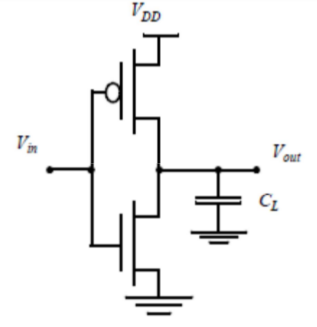
\includegraphics[width=0.35\textwidth]{C3_1.png}\\
\raggedright

We will refer to CMOS inverter implemented in a static FC-CMOS logic. FC-COMS means fully-complementary logic, which is a particular class of static gates.
Static refers to the fact that these gates have an output node always connected to GND or VDD through a low impedance path. Fully-complementary means that the gate is composed by a pull-down network and a complementary pull-up network.\\

\section{Static behavior}

Independently of the transistor size the high and low output levels are equal to $V_{DD}$ and GND that in out reference technology are 2.5V and 0V
\begin{equation}
V_{OH}=V_{DD}=2.5V
\end{equation}
\begin{equation}
V_{OL}=GND=0V
\end{equation}
This two values are indipentent form the relative device size; gates with this propriety are called ratioless (gates without this propriety are ratioead).\\
\vspace{5mm}
There is always in steady state a finite resistance between the output node and GDN or VDD (that isn't the equivalent resitance of the previous chapter that is useful to assest the propagation delay).\\
For VDD=2.5V we get
\begin{equation}
r_{on}=\frac{4.2k}{(W/L)_n}\ \ \ \ \ \ \ \ \ \ r_{on}=\frac{15.9k}{(W/L)_p} 
\end{equation}

\centering
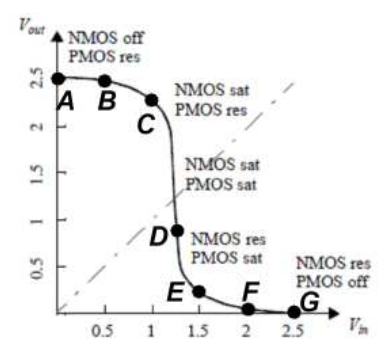
\includegraphics[width=0.35\textwidth]{C3_2.png}\\
\raggedright



\subsection{Switching threshold}
Let's suppose that during the transistion both transistor are in velocity saturation region (this is not correct but leads to a negligible error) to assest the threshold voltage $V_M$ of the inverter we have to put the 2 currents of the mos equal doing this we obtain 

\vspace{2.5mm}

\centering
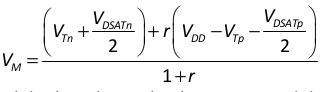
\includegraphics[width=0.35\textwidth]{C3_3.png}\\
\raggedright
 
with 

\centering
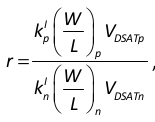
\includegraphics[width=0.15\textwidth]{C3_4.png}\\
\raggedright

We can oslo have the following inverse relationship

\vspace{2.5mm}

\centering
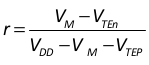
\includegraphics[width=0.15\textwidth]{C3_5.png}\\
\raggedright

For $V_M=1.25V$ that is the best case we get
\begin{equation}
\frac{(W/L)_p}{(W/L)_n}=3.5\simeq 3
\end{equation}

\subsection{Noise marigns}

To compute $V_{IL}$, $V_{IH}$ we consider the piecewise linear approximation for the VTC, where the transition region is approximated by a straight line having the same negative slope of original VTC in the threshold point.\\

\centering
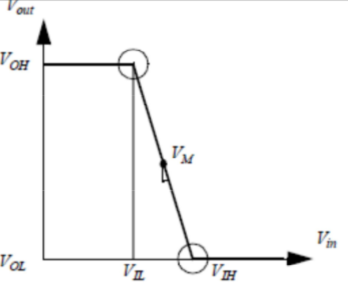
\includegraphics[width=0.35\textwidth]{C3_6.png}\\
\raggedright

In this way the straight line that approximates the VTC near the threshold is 
\begin{equation}
V_{OUT}=V_{IN}g+(1-g)V_M \ \ \ \ \ \ (g<0)
\end{equation}
we can compute g considering that $g=-(g_{mn}+g_{mp})r_{0p}//r_{0p}$ we obtain

\vspace{2.5mm}

\centering
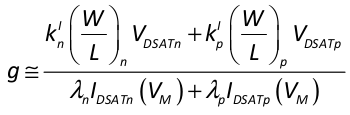
\includegraphics[width=0.35\textwidth]{C3_7.png}\\
\raggedright

\vspace{2.5mm}

The gain is apporoximately constant if the velocity saturation is taken into account.\\

From this we get 

\centering
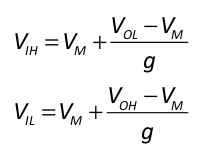
\includegraphics[width=0.15\textwidth]{C3_8.png}\\
\raggedright

\centering
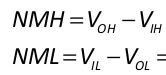
\includegraphics[width=0.11\textwidth]{C3_9.png}\\
\raggedright

\section{Dinamic behavior}


\centering
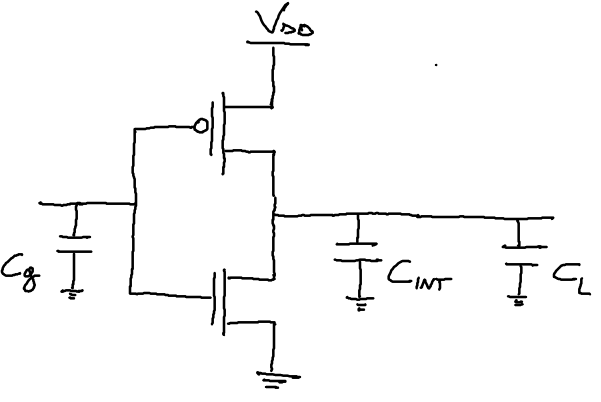
\includegraphics[width=0.45\textwidth]{C3_10.png}\\
\raggedright

We define the following parameters \\
\tab $W_n,W_p$ the width of the drain junctions (that is the same of W/L)\\
\tab $L_D$ Drain length (that isn't the same as W/L)\\
\tab $A_{d}=W*L_D$ the area of the drain\\
\tab $P_{d}=2L_D+W$ the perimeter of the drain\\


\subsection{Intinsic capacitance $C_{int}$}
\vspace{2mm}
\begin{equation}
C_{int}=C_{overlap}+C_{dbn}+C_{dbSWn}+C_{dbp}C_{dbSWp}
\end{equation}
{\bf Overlap capacitance}\\
\begin{equation}
C_{ovelap}=2(C'_{ovp}W_p+C'_{ovn}W_n)
\end{equation}
\vspace{5mm}
{\bf Drain-bulk n capacitances}
\begin{equation}
C_{dbn}=\frac{C'_{jn}A_{dn}}{2}\left(\frac{1}{(1+\frac{V_{DD}}{\phi})^{0.5}}+\frac{1}{(1+\frac{V_{DD}}{2\phi})^{0.5}}  \right)
\end{equation}

\begin{equation}
C_{dbSWn}=\frac{C'_{jSWn}P_{dn}}{2}\left(\frac{1}{(1+\frac{V_{DD}}{\phi})^{0.44}}+\frac{1}{(1+\frac{V_{DD}}{2\phi})^{0.44}}  \right)
\end{equation}

\vspace{5mm}
{\bf Drain-bulk p capacitances}
\begin{equation}
C_{dbp}=\frac{C'_{jp}A_{dp}}{2}\left(1+\frac{1}{(1+\frac{V_{DD}}{2\phi})^{0.48}}  \right)
\end{equation}

\begin{equation}
C_{dbp}=\frac{C'_{jSWp}P_{dp}}{2}\left(1+\frac{1}{(1+\frac{V_{DD}}{2\phi})^{0.32}}  \right)
\end{equation}


\subsection{Gate capacitance $C_{g}$}

\begin{equation}
C_g=C'_{ovn}W_n+C'_{ovp}W_p+C'_{ox}(W_nL_n+W_pL_p)
\end{equation}

\subsection{Self-loading factor}
We can define the self-loading factor $\gamma$ as 
\begin{equation}
C_{int}=\gamma C_g
\end{equation}
In our reference technology we have $\gamma=1$ and $C_g^{(1)}=2fF$ where the suffix (1) is the size of the inverter (that is the W/L of the n-mos).\\
If we have an inverter of size $\alpha$ it's gate capacitance will be 
\begin{equation}
C_g^{(\alpha)}=\alpha C_g^{(1)}=\alpha\cdot 2fF
\end{equation}


\section{Propagation delay}
\centering
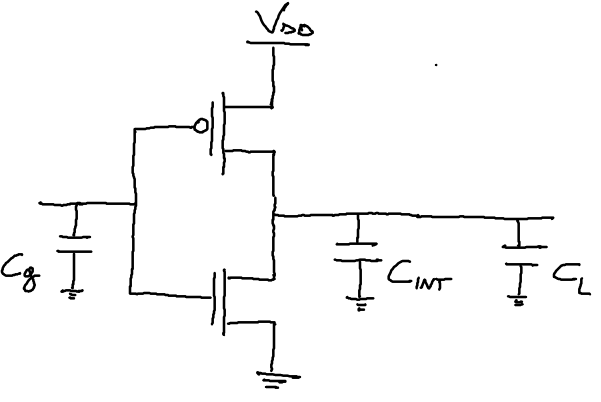
\includegraphics[width=0.45\textwidth]{C3_10.png}\\
\raggedright

Propagation delay form high to low

\centering
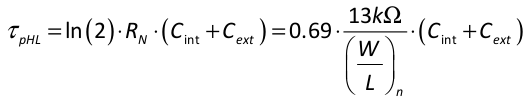
\includegraphics[width=0.35\textwidth]{C3_11.png}\\
\raggedright

\vspace{5mm}

Propagation delay forom low to high 

\centering
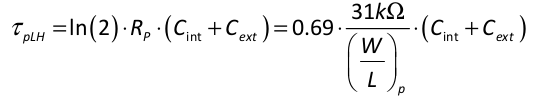
\includegraphics[width=0.35\textwidth]{C3_12.png}\\
\raggedright

\vspace{5mm}
We define intrinsic propagation delay as the average between this 2 results when $C_{ext}=0$
\begin{equation}
\tau_{p0}=\frac{\tau_{HL}+\tau_{LH}}{2}
\end{equation}

\subsection{Fan-out}
Considering an external capacitance we get the folowing expression
\begin{equation}
\tau_p=\ln(2)R_{eq}(C_{int}+C_{ext})=\tau_{p0}\left(1+\frac{C_{ext}}{C_{int}}\right)=\tau_{p0}\left(1+\frac{C_{ext}}{\gamma C_g}\right)=\tau_{p0}\left(1+\frac{f}{\gamma}\right)
\end{equation}
Where we used the fan-out f and the self-loading factor defined as
\begin{equation}
f=\frac{C_{ext}}{C_g}\ \ \ \ \ \ \ \ \ \ \ \ C_{int}=\gamma C_g
\end{equation}

\section{Chain of inverters}

To optimize the propagation delay of an inverter chain with N elements we have to set all propagation delay of the inverters equal $f_i=f_i+1\ \ \  \forall i=0,...,N$.\\
To do this we have to calculate the path fan-out that is the load over the first gate capcitance
\begin{equation}
F=\frac{C_L}{C_{g,1}}
\end{equation} 
And from this we calculate the optimum fan-out 
\begin{equation}
f_{opt}=\sqrt[N]{F}
\end{equation}
given the first inverter size $s_1$ all the other inverters' dimensions are fixed 
\begin{equation}
s_n=s_1\cdot (f_{opt})^{n} \ \ \ \forall n=1,...,N 
\end{equation} 
and the propagation delay is 
\begin{equation}
\tau_p=N\tau_{p0}\left(1+\frac{f_{opt}}{\gamma} \right)
\end{equation}

\vspace{5mm}

If the number of inverter isn't fixed we can compute for our reference technology the optimum number of stages as 
\begin{equation}
N_{opt}=\frac{\ln(F)}{\ln(3.6)}
\end{equation}
beacuse the best fan-out that we can have is 
\begin{equation}
f_{opt}^{ideal}=3.6
\end{equation}
Of course the number of stages N has to ben an integer number.\\

